\section{A Model for DevOps Adoption}\label{sec:case_study}

Based on H1-H4 hypothesis, we present a three step model that
explains how to adopt DevOps according to our understanding. The
model considers the following steps:

\begin{enumerate}
\item In the first step, a company should
  \textbf{disseminate the relevance of building a collaborative} culture between
  development and operations teams, as the main
  goal of a DevOps effort.

\item In the second step, a company should \textbf{select and develop
the most suitable enablers} according to its context. The enablers
are means commonly used to develop the collaborative culture and its concepts.

\item In the third step, a company should \textbf{check the outcomes of the
DevOps adoption} in order to verify the alignment with
industrial practices and to explore them according to the company's need.
\end{enumerate}

Figure~\ref{model} illustrates the categories and the
relationships according to the hypothesis. The proposed model is built upon
the hypothesis and is one of possible applications of the theory. It was proposed
assuming that following the patterns identified in companies that were
well succeeded in DevOps adoption can be a good way to reduce the risks of
failure during the process.

\begin{figure}[bht]
  \centering
  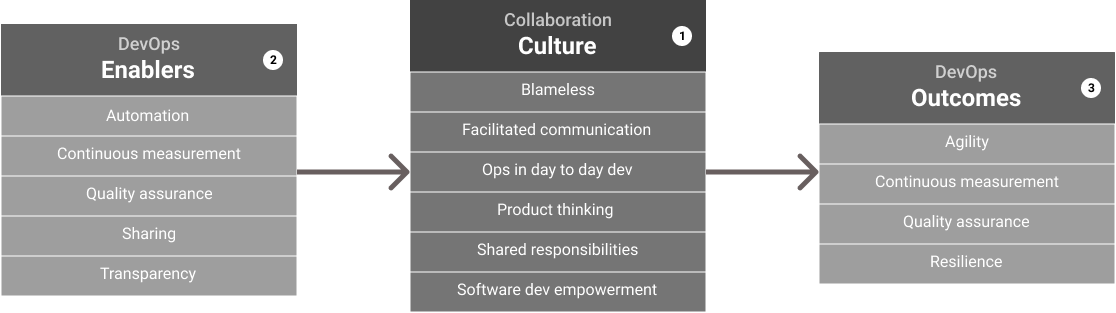
\includegraphics[width=.75\textwidth]{model.png}
  \caption{Categories and Relationships. Categories label with a * means
    thant they are within both \emph{enabler} and \emph{expected
    outcomes} categories.}
  \label{model}
\end{figure}


Our proposed model has been applied to guide the DevOps adoption at the
Brazilian Federal Court of Accounts (TCU) where one of the authors of this study
works as a software developer. In the next we present the details about the DevOps
adoption at TCU and explain the applicability and relevance of our model in a
practical scenario.
